\section{Experiments and Results}
We use transactional data from instacart kaggle challenge to train all our models. As can 
be seen in Figure~\ref{fig:sampledata} data has transactional details including consumer id, item id, 
order id, add to cart order, date of transaction, aisle id and department id.
Also, from Table 1, we can see that we utilize 1 year data which gets split into train, validation,
test1 and test2. We generate consumer-item-week level data with purchase/ non purchase being the target.
We use the above data to generate consumer-item purchase predictions for forwards 2 time steps (2 weeks for our case).
 \begin{figure*}[!t]
    \centering 
    \caption{Sample Dataset} 
    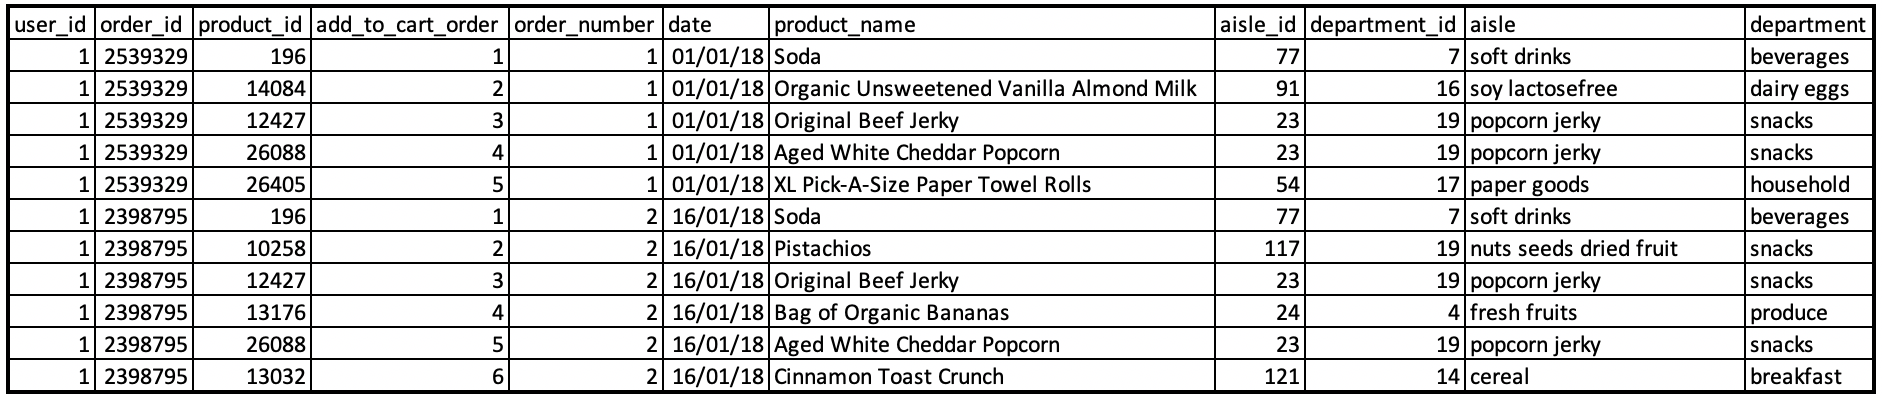
\includegraphics[width=6.6in]{img/sampledata.png} 
    \label{fig:sampledata} 
  \end{figure*}

  \begin{figure}[t]
    \centering 
    \caption{Most ordered Items across Departments} 
    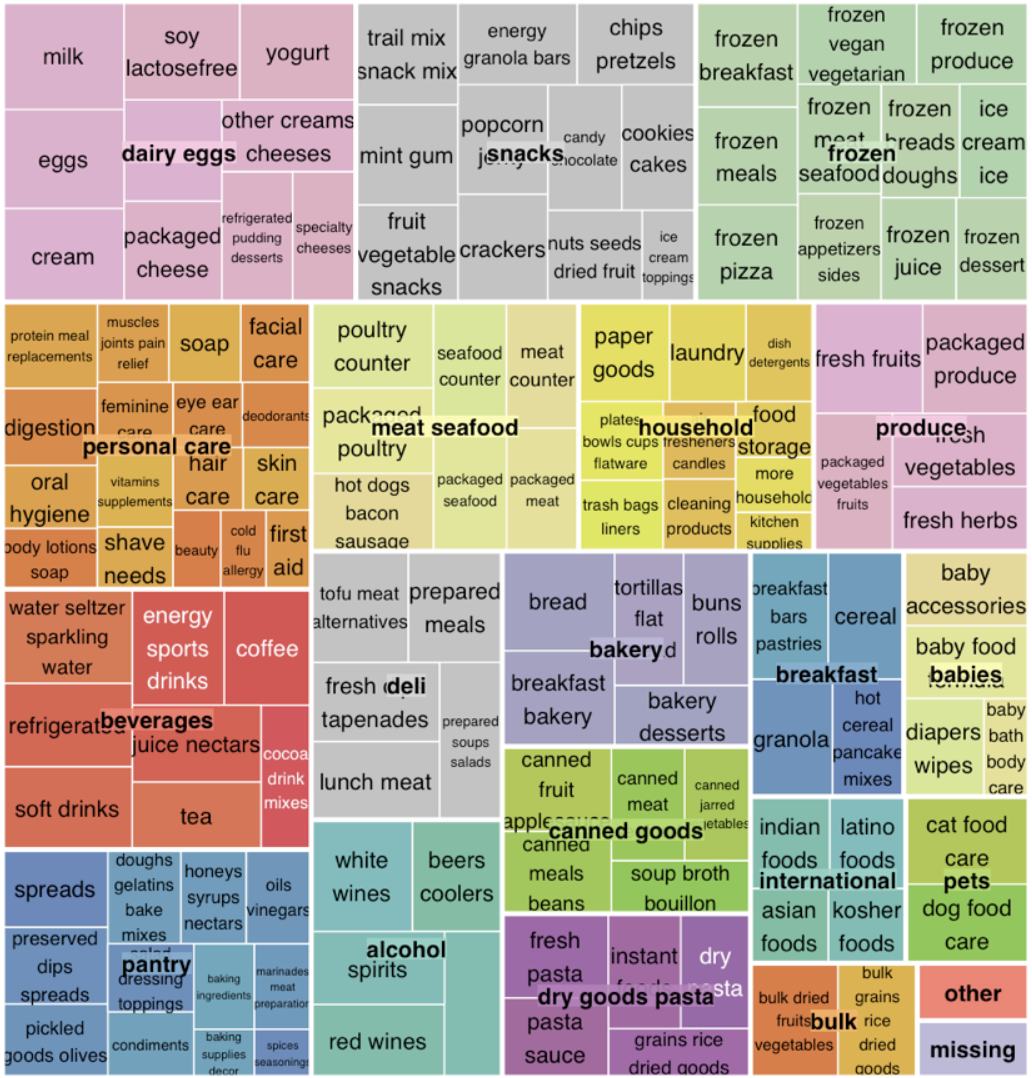
\includegraphics[width=2.5in]{img/items.png} 
    \label{fig:items} 
  \end{figure}

  \begin{figure}[t]
    \centering 
    \caption{Density of consumers Vs. Basket Size} 
    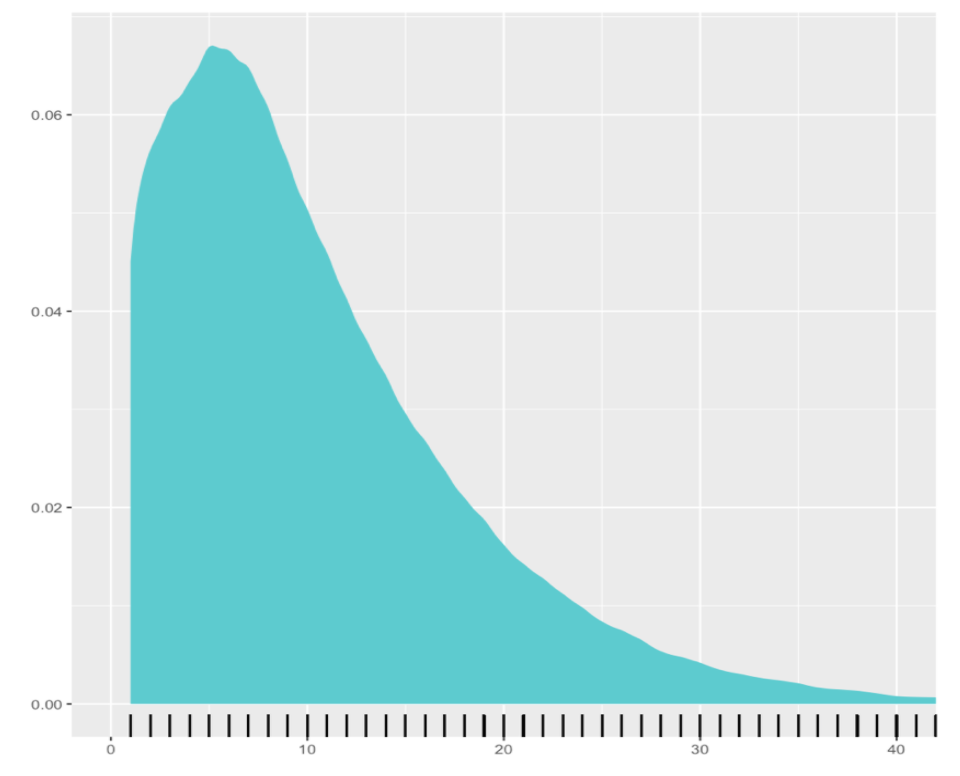
\includegraphics[width=2.5in]{img/basket.png} 
    \label{fig:basket} 
  \end{figure}

  \begin{figure}[t]
    \centering 
    \caption{Order probability Vs. Add to cart order} 
    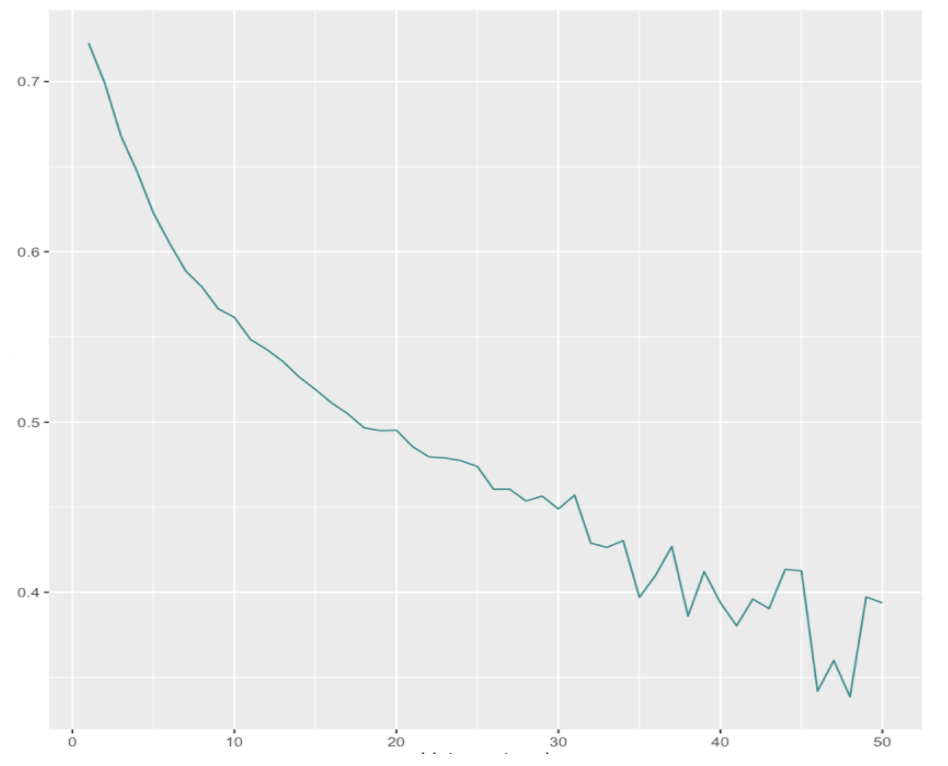
\includegraphics[width=2.5in]{img/addtocart.png} 
    \label{fig:addtocart} 
  \end{figure}

\begin{center}
\begin{table*}[!t]
\caption{BCELoss of Test2 for 12 Trials of Deep Learning Models} 
\centering
\resizebox{\textwidth}{!}{\begin{tabular}{|r|l|r|r|r|r|r|r|r|}
  \hline
 {\bf Trial} & {\bf Optimizer} & {\bf Scheduler} & {\bf SWA} & {\bf Parameter Avg} &  {\bf MLP} & {\bf LSTM} 
 &  {\bf TCN} & {\bf TCN-LSTM} \\ [0.5ex] 
  \hline\hline
1 & RMSprop & ReduceLROnPlateau & True & False &  {\bf 0.0276} & 0.0306 & {\bf 0.0249} & 0.0307 \\ 
2 & RMSprop & CyclicLR & True & False &  0.0708 & {\bf 0.0269} & {\bf 0.0269} & 0.0348 \\ 
3 & Adam & ReduceLROnPlateau & True & False &  0.0295 & 0.0303 & 0.0667 & 0.0337 \\ 
4 & RMSprop & ReduceLROnPlateau & False & False &  0.2427 & {\bf 0.0275} & 0.0364 & 0.0759 \\ 
5 & RMSprop & CyclicLR & False & False &  {\bf 0.0250} & 0.0306 & 0.0600 & {\bf 0.0286} \\ 
6 & Adam & ReduceLROnPlateau & False & False&  0.0360 & {\bf 0.0302} & 0.0590 & 0.0309 \\ 
7 & RMSprop & ReduceLROnPlateau & False & True &  0.2903 & 0.0432 & 0.0453 & 0.0381 \\ 
8 & RMSprop & CyclicLR& False & True &  {\bf 0.0245} & 0.0378 & 0.0569 & {\bf 0.0262} \\ 
9 & Adam & ReduceLROnPlateau & False & True & 0.0700 & 0.0491 & 0.0610 & 0.0382 \\ 
10 & RMSprop & ReduceLROnPlateau & True & True & 0.0356 & 0.0364 & {\bf 0.0238} & 0.0309 \\ 
11 & RMSprop & CyclicLR & True & True &  0.0420 & 0.0377 & 0.0284 & {\bf 0.0269} \\ 
12 & Adam  & ReduceLROnPlateau & True & True&  0.0321 & 0.0306 & 0.0547 & 0.0305 \\ [1ex] 
   \hline
\end{tabular}}
\end{table*} 
\end{center}

\begin{table}[t]
\caption{BCELoss of Test2 for 6 best Trials of ML Models}
\vspace{0.1 in}
\centering
\resizebox{3.3in}{!}
{%
\begin{tabular}{|c|c|c|c|c|}
\hline
{\bf Trial} & {\bf Hyper-Parameter} & {\bf Xgboost} & {\bf RandomForest} \\  
\hline\hline
1  		&  Bayesian-Optimizer &  {\bf 0.0332} &  0.0526   \\ 
2	  		&  Bayesian-Optimizer &  0.0364 &  0.0479   \\ 
3  		&  Bayesian-Optimizer &  0.0347 &  {\bf 0.0416}  \\ 
4	  		&  Bayesian-Optimizer &  0.0364 &  {\bf 0.0449}  \\ 
5	  		&  Bayesian-Optimizer &  {\bf 0.0335} &  {\bf 0.0459}  \\ 
6	  		&  Bayesian-Optimizer &  {\bf 0.0339} &  0.0578  \\ 
\hline
\end{tabular}
}
\label{tab:mlmodels}
\end{table}


\begin{table}[t]
\caption{ BCELoss mean of top 3 trials across data splits}
\vspace{0.1 in}
\centering
\resizebox{3.3in}{!}
{%
\begin{tabular}{|c|c|c|c|c|}
\hline
{\bf Model Type} & {\bf Val BCELoss} & {\bf Test1 BCELoss} & {\bf Test2 BCELoss} \\ 
\hline\hline 
MLP	  		&  0.0405 &  0.0289 &  0.0256  \\ \hline
LSTM  		&  0.0373 &  0.0293 &  0.0282 \\ \hline
{\bf TCN}			&  {\bf 0.0368}  &  {\bf 0.0292} &  {\bf 0.0251}  \\ \hline
TCNLSTM 	& 0.0368  & 0.0304	& 0.0273	 \\ \hline
Xgboost 	& 0.0352 & 0.0318	& 0.0335	\\ \hline
RandomForest & 0.0437 & 0.0389	& 0.0441	\\ \hline
\end{tabular}
}
\label{tab:training}
\end{table}


\begin{table}[t]
\caption{ Stacked Generalization Results}
\vspace{0.1 in}
\centering
\resizebox{3.3in}{!}
{%
\begin{tabular}{|c|c|c|c|c|c|}
\hline
{\bf Model Type} & {\bf K Value} & {\bf Val BCELoss} & {\bf Test1 BCELoss} & {\bf Test2 BCELoss} \\ 
\hline\hline 
{\bf Weighted K Best}	  &  {\bf 3}  &  {\bf 0.0386} &  {\bf 0.0278} &  {\bf 0.0242}  \\ \hline
Weighted K Best	  		&  5  &  0.0373 &  0.0282 &  0.0245  \\ \hline
Weighted K Best	  		 &  10 &  0.0397 &  0.0290 &  0.0258  \\ \hline
Weighted K Best	  		 &  15 &  0.0389 &  0.0296 &  0.0272  \\ \hline
Weighted K Best	  		&  25  &  0.0394 &  0.0316 &  0.0287  \\ \hline
\end{tabular}
}
\label{tab:stacking}
\end{table}

  \begin{figure}[t]
    \centering 
    \caption{Probability Distributions} 
    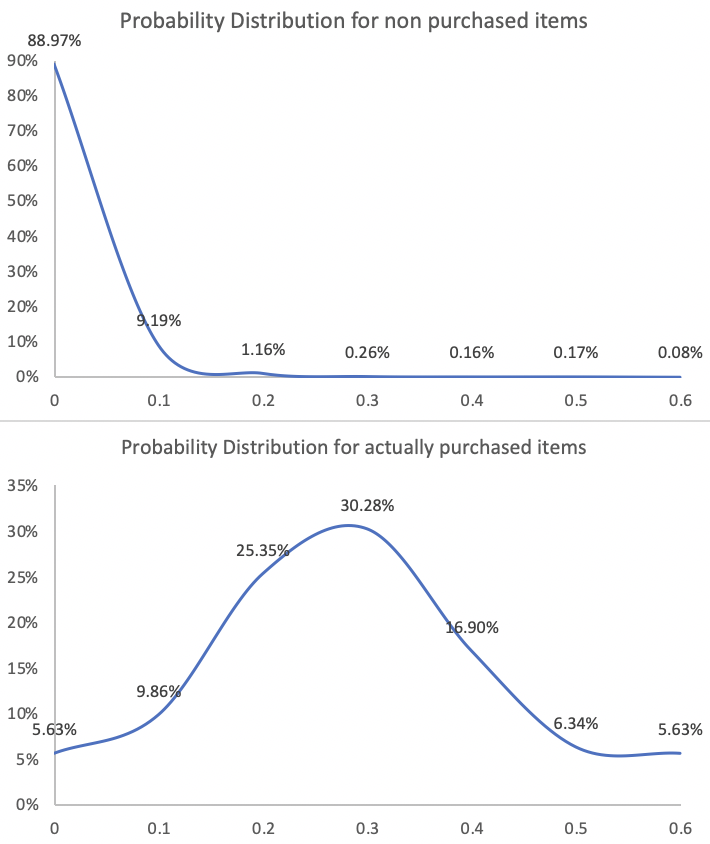
\includegraphics[width=3.3in]{img/density.png} 
    {\bf Probability Distributions for the non purchased cases tends towards 0 and tapers as the 
    probability moves towards 0.5, whereas for purchased cases the distribution witnesses a peak 
    between 0.2 and 0.3

    purchased cases  0.5} 
    \label{fig:density} 
  \end{figure}

\begin{table}[t]
\caption{Final Accuracy post F\textsubscript{1}-Maximization}
\vspace{0.1 in}
\centering
\resizebox{3.3in}{!}
{%
\begin{tabular}{|c|c|c|c|}
\hline
{\bf Data Split} & {\bf Precision} & {\bf Recall} & {\bf F\textsubscript{1}-Score} \\ 
\hline\hline 
Validation	  	 &  0.3401 &  0.4981 &  0.4042  \\ \hline
Test1	  		 &  0.3323 &  0.5103 &  0.4024  \\ \hline
Test2	  		 & 0.3506 &  0.4964 &  0.4109 \\ \hline
\end{tabular}
}
\label{tab:Fscore}
\end{table}

\subsection{Experimental setup}
We started with exploratary data analysis, looking at the data from various cuts and 
trying to study the variations of the features with target. Some of them include looking at the 
density of consumers with different basket sizes Figure~\ref{fig:basket}, orders placed for items 
across departments Figure~\ref{fig:items}, variation of order probability with add to cart order Figure~\ref{fig:addtocart},
order probability variations at different temporal cuts like week, month and quarter, transactional metrics at both
consumer and item levels like total orders, total reorders, recency, gap between orders, etc.
We then performed multiple experiments with above features and different hyper-configurations.

\subsection{Results and Observations}
Tables 3 and 4 shows the experimental results obtained with different hyper-configurations over multiple models.
From Table 3, we can infer that RMSprop and CyclicLR emerged as the clear winners as 
Optimizer and Scheduler respectively. TCN showed the best Accuracy score at test2, with most of the other Deep
Learning models have comparable results. Also, we observe that all the Deep Learning models out perform Machine Learning 
models including Xgboost and RandomForest both in terms of Accuracy and Generalization. This insight can be drawn from 
table 5 which has the average of BCELoss across 3 best trials. Range of scores across val , test1 and test2 states 
that Deep Learning models are showing more stable results in terms of model fit. 
We present the effectiveness of combining predictions in the form of stacking. From Table 6, we can see the 
results of stacking at different values of K, both for Weighted K-Best as well as K-Best model setups. Finally we 
apply F\textsubscript{1}-Maximization so as to be able to strike a balance between Precision and Recall.
After F\textsubscript{1}-Maximization we see that all Precision, Recall and F\textsubscript{1}-Score 
are close enough for all data splits as can be seen from Table 7.
\subsection{Industrial Applications}
The Next Logical Purchase framework has multiple applications in retail industry. Some of its applications 
include:
\begin{itemize}
\item {\bf Consumer-Item Recommendation:} Item Recommendations at consumer level can be derived from the 
solution of this problem, which will enhance consumer shopping experience.
\item {\bf Inventory Planning:} This can help in Planning inventory well, as it provides the 
consumer choice at a point time.
\item {\bf Assortment Planning:} In retail stores, this can be used for placing items in MOD based on the 
consumer preference model at a given time frame.
\end{itemize}
